It should be noted that we could not use the MSCTD dataset completely, since some scenes did not have a person in them, (for face or pose recognition), or their face and/or pose could not be recognized. Due to these problems, first, we filtered this dataset, which led to omitting about 20 percent of MSCTD, and then it was used for our model.
\paragraph{} In order to create a multi-modal network, we decided to extract two embeddings from pre-trained networks, then concatenate them and add a linear layer, which leads to a classifier with three possible outcomes for existing sentiments  (i.e., positive/ neutral/ negative). We compared the result of this classifier with single-modal networks with a number of criteria. 

\subsection{Text Classifier}
We used the "RobertaForSequenceClassification" classifier based on RoBERTa~\cite{liu2019roberta}, a robustly optimized method for pretraining NLP systems that improves on BERT, the self-supervised method released by Google, which gives us the sentiment of a text. Sequence classification uses the final embedding for \textit{CLS} token of each sentence. Its details can be seen in Figure~\ref{fig:CLS}. \textit{MSCTD} dataset's scripts are classified by this pre-trained network. 

\begin{figure}[t]
	\centering
	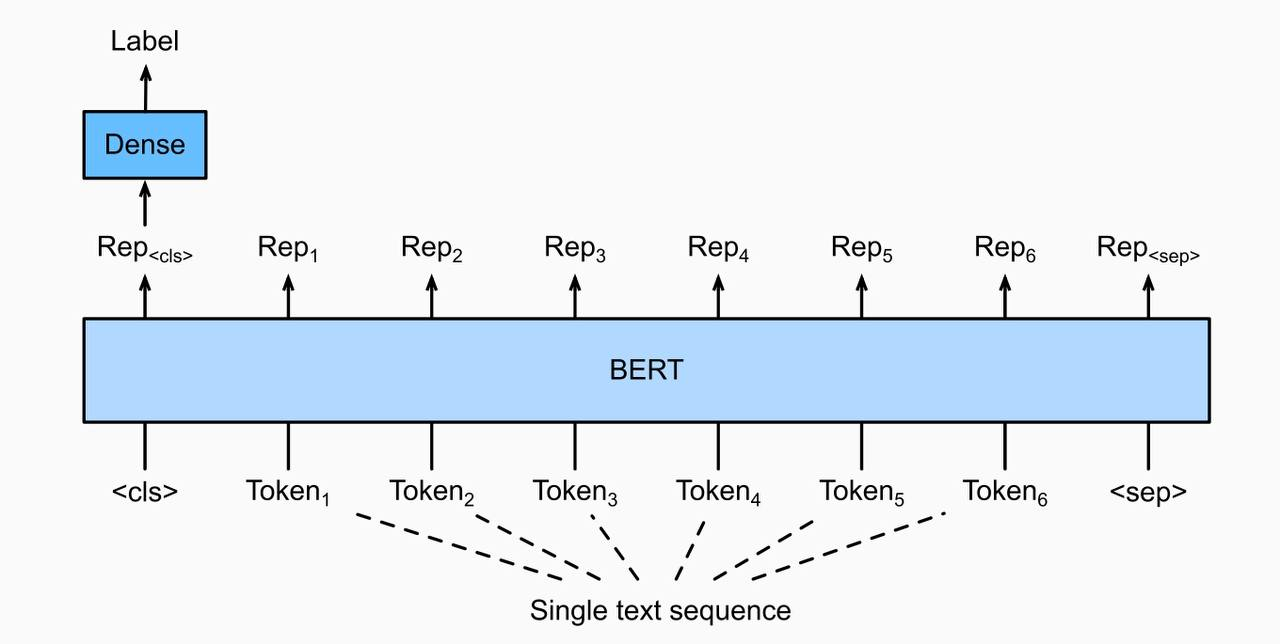
\includegraphics[width=\linewidth]{fig/CLS}
	\caption{Roberta For Sequence Classification}
	\label{fig:CLS}
\end{figure}

\subsection{Image Classifier}

\paragraph{Face recognition} In order to extract a face from an image, four steps must be done:

\begin{enumerate}
	%Face detection
	\item\label{item:1}\emph{Face detection}: We used the \textit{MTCNN}~\cite{zhang2016joint} implemented with facenet pytorch (since it was much faster than implemented with TensorFlow) in order that the fundamental face points, such as eyes, nose, mouth, etc. are determined.
	%Face alignment
	\item\label{item:2}\emph{Face alignment}: All faces should be aligned, using the angle of eyes with a horizontal line. As a result, all face points will be in similar conditions after this rotation.\\\textit{MTCNN} can detect and align the face in three stages: In the first stage it uses a shallow CNN to quickly produce candidate windows. In the second stage it refines the proposed candidate windows through a more complex CNN. And lastly, in the third stage it uses a third CNN, more complex than the others, to further refine the result and output facial landmark positions.
	%Landmark detector
	\item\label{item:3}\emph{Landmark detector}: With some help from the \textit{Dlib} library~\cite{kazemi2014one} in order to find landmarks around the face, we masked the face and removed extra points out of the face. By doing this, emotion recognition from the face will be more precise. After localizing the face in the image, detecting these landmarks will be possible. With this pre-trained facial landmark detector, 68 (x, y) coordinates of facial structures will be estimated and those of them which are around the face and specify its boundary will be used.
	%Emotion recognition
	\item\label{item:4}\emph{Emotion recognition}: The sentiment of a face will be recognized using a model called \textit{Multi-task EfficientNet-B2}~\cite{savchenko2022classifying}, by a single efficient neural network. This network is pre-trained on face identification and fine-tuned for facial expression recognition on static images. At the end of this network, there is a sub-network for classifying the emotion, based on its input which is emotion embedding. As we decided to keep this embedding in order to combine it with other embeddings, this sub-network is omitted. 
\end{enumerate}

After all these steps, the last layer's features of the dense model will be used as an embedding for a face. By this method, the embedding of each face can be extracted. Moreover, getting the average of all face embeddings is also possible.

\paragraph{Pose detection} As an improvement, we decided to include the pose of humans in our model, using keypoint extraction~\cite{xiao2018simple}. By this method, 17 (x, y) keypoints' coordinates of a person, such as elbows and ears, in a frame will be detected and concatenated. This method is based on a few deconvolutional layers added to a backbone network, which is ResNet-50.

\paragraph{Scene recognition} We used a model which its backbone is ResNet-50 to extract an embedding for each scene and added this embedding to the previous ones, although scene details did not improve our accuracy in recognizing emotion from a frame. As a result, we found out that a scene on its own does not have any additional information about sentiment. Perhaps a scene in which its faces have been masked includes extra data, but we did not try this method and we trained our model with scenes with faces.

%Now comes the "beef" of the paper, where you explain what
%you did. Again, organize it in paragraphs with titles. As in
%every section you start with a very brief overview of the
%section. 
%
%This section may vary significantly depending on your topic.
%You may also choose to make the different parts individual sections.
%Here is a more general structure:
%
%\subsection{Design} Concisely present your design. Focus on novel aspects,
%but avoid implementation details. Use pseudo-code and figures to better
%explain your design, but also present and explain these in the text.
%%
%To assist in evaluating your design choices, it may be relevant to describe
%several distinct \textit{design alternatives} that can later be compared.
%
%\subsection{Analysis} Argue for the correctness of your design and 
%why you expect it to perform better than previous work.
%%
%If applicable, mention how your design relates to theoretical bounds.
%
%\subsection{Optimization} Explain how you optimized your design and 
%adjusted it to specific situations.
%%
%Generally, as important as the final results is to show
%that you took a structured, organized approach to the optimization
%and that you explain why you did what you did.
%%
%Be careful to argue, why your optimization does not break the 
%correctness of your design, established above.
%%
%It is often a good strategy to explain a design or protocol in stepwise refinements,
%so as to more easily convince the reader of its correctness. 
%
%\subsection{Implementation} It is not necessary to "explain" your code. 
%However, in some cases it may be relevant to highlight 
%additional contributions given by your implementation.
%Examples for such contributions are:
%\begin{itemize}
%\item \emph{Abstractions and modules}: If your implementation is nicely separated into interacting
%modules with separated responsibilities you could explain this structure,
%and why it is good/better than some other alternative structure.
%\item \emph{Optimization}: If you spend significant time optimizing your code, e.g.~using profiling tools,
%the result of such optimization may be presented as a contribution. In this case, reason, 
%why the optimized code works better.
%\item \emph{Evaluation framework}: If you implemented a framework or application to evaluate your implementation against existing work, or in a specific scenario, this framework may be presented as a contribution.
%\end{itemize}
%
%Make sure to cite all external resources used.
